%----------------------------------------------------------------------------------------
%	SOLUTION 4
%----------------------------------------------------------------------------------------
\subsection*{Solution 4}
\paragraph{Logistic regression (LR):} Let $N, K, x\in \mathbb{R}^d, C_i, w_i \in \mathbb{R}^d, w_{i0} \in \mathbb{R}$ denote number of samples, number of classes, data sample, $i^{th}$ class, weights and intercept of the linear model respectively. For logistic regression, I use the $softmax$ function, as shown below, to find the posterior:
\begin{align*}
y_i = \hat{P}(C_i | x) = \frac{\text{exp}[w_i^Tx + w_{i0}]}{\sum_{j=1}^K\text{exp}[w_j^Tx + w_{j0}]},
\end{align*}
for all $i \in \{1,2,\ldots, K\}$. The error function is
\begin{align*}
E = -\sum_{t=1}^N \sum_{i=1}^K r_i^t \log(y_i),
\end{align*}
where $r_i^t = 1$ if $x^t \in C_i$ and $0$ otherwise. The objective is to find optimal values of $w_i, w_{i0}$ for all $i \in \{1,2,\ldots,K\}$ such that the error $E$ is minimized. I use gradient descent to find the updates to $w_i, w_{i0}$. The gradient of $E$ with respect to $w_i$ is
\begin{align*}
\frac{\partial E}{\partial w_i} &= \frac{\partial E}{\partial y_i} \frac{\partial y_i}{\partial w_i}\\
&= -\sum_{t=1}^N(r_i^t - y_i^t)x^t,
\end{align*}
and
\begin{align*}
\frac{\partial E}{\partial w_{i0}} &= \frac{\partial E}{\partial y_i}\frac{\partial y_i}{\partial w_{i0}}\\
&= -\sum_{t=1}^N(r_i^t - y_i^t).
\end{align*}
Therefore, the update equation for gradient descent algorithm is
\begin{align*}
w_i^{new} &= w_i^{old} + \eta \sum_{t=1}^N(r_i^t - y_i^t)x^t,\\
w_{i0}^{new} &= w_{i0}^{old} + \eta \sum_{t=1}^N(r_i^t - y_i^t),
\end{align*}
where $\eta$ is the learning rate. I have taken $\eta=0.001$. I have also kept a provision to add regularization term in my code for which the update equation becomes,
\begin{align*}
w_i^{new} &= w_i^{old} + \eta \sum_{t=1}^N(r_i^t - y_i^t)x^t -\eta C w_i^{old},\\
w_{i0}^{new} &= w_{i0}^{old} + \eta \sum_{t=1}^N(r_i^t - y_i^t) - \eta C w_{i0}^{old},
\end{align*}
where $C$ is the regularization term which I have taken as $10$ in my code. I have used batch gradient descent.
\paragraph{Naive Bayes with marginal Gaussian distributions (GNB):} In case of Naive Bayes, we assume that the features in the samples are uncorrelated. Therefore, the covariance matrices are diagonal. The approach is similar to as described in Solution 3.ii. But to compare GNB to linear LR, we need to make use of shared covariance matrix for all classes. Therefore, we can use pooling of data to find a shared covariance matrix as follows
\begin{align}
	S = \sum_{i=1}^K \hat{P}(C_i)S_i,
\end{align}
where $\hat{P}(C_i), S_i$ are defined in~(\ref{eq:mle}). Now, if we use $S$ in place of $S_i$ for all $i \in \{1,2,\ldots,K\}$ in~(\ref{eq:disc_func}), we can see that the term $-\frac{1}{2}\log(|S|)$ becomes common to all discriminators. Therefore, we can drop this term and use
\begin{align*}
	g_i(x) = -\frac{1}{2}(x-m_i)^TS^{-1}(x-m_i) + \log(\hat{P}(C_i)).
\end{align*}
as the discriminator. In this case, we see that the quadratic term $\frac{1}{2}x^TS^{-1}x$ becomes common to all discriminators, thus, the discriminator gives rise to a linear function of $x$ which can be compared to LR model.
\paragraph{Results:} Fig.~\ref{fig:boston50_test_err}, Fig.~\ref{fig:boston75_test_err} and Fig.~\ref{fig:digits_test_err} show the test data error percentage for LR anf GNB model, for `Boston50', `Boston75' and `Digits' data respectively, with percentage of training data used to train the model in x-axis. It can be seen that the LR model performs better than GNB.
\begin{figure}[h]
	\centering
	\subfloat[][Test set error plot on Boston50 dataset]{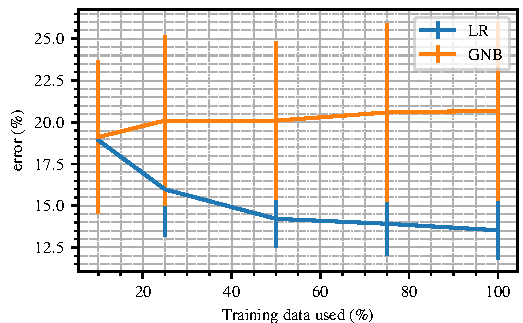
\includegraphics[scale=1.0,trim={0cm 0cm 0cm 0cm},clip]{./code/generatedPlots/Q4_boston50_test_err.pdf}
	\label{fig:boston50_test_err}}\hspace*{0.5cm}
	\subfloat[][Test set error plot on Boston75 dataset]{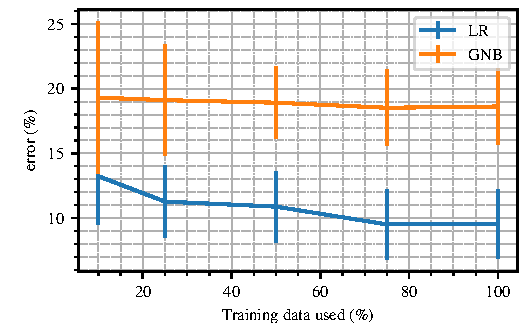
\includegraphics[scale=1.0,trim={0cm 0cm 0cm 0cm},clip]{./code/generatedPlots/Q4_boston75_test_err.pdf}
	\label{fig:boston75_test_err}}\\
	\subfloat[][Test set error plot on digits dataset]{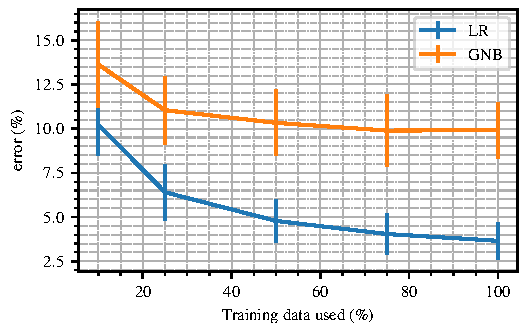
\includegraphics[scale=1.0,trim={0cm 0cm 0cm 0cm},clip]{./code/generatedPlots/Q4_digits_test_err.pdf}
	\label{fig:digits_test_err}}
	\caption{Q4: Test data error comparison between LR and GNB}
\end{figure}
